\subsubsection{Diffusjon}
Et n-type stoff ved siden av et p-type stoff, fører til diffusjon.
De svakt bundede elektronene i n-type swoopper over
til hullene i p-type.
Dette kalles \emph{diffusjon}.
\\
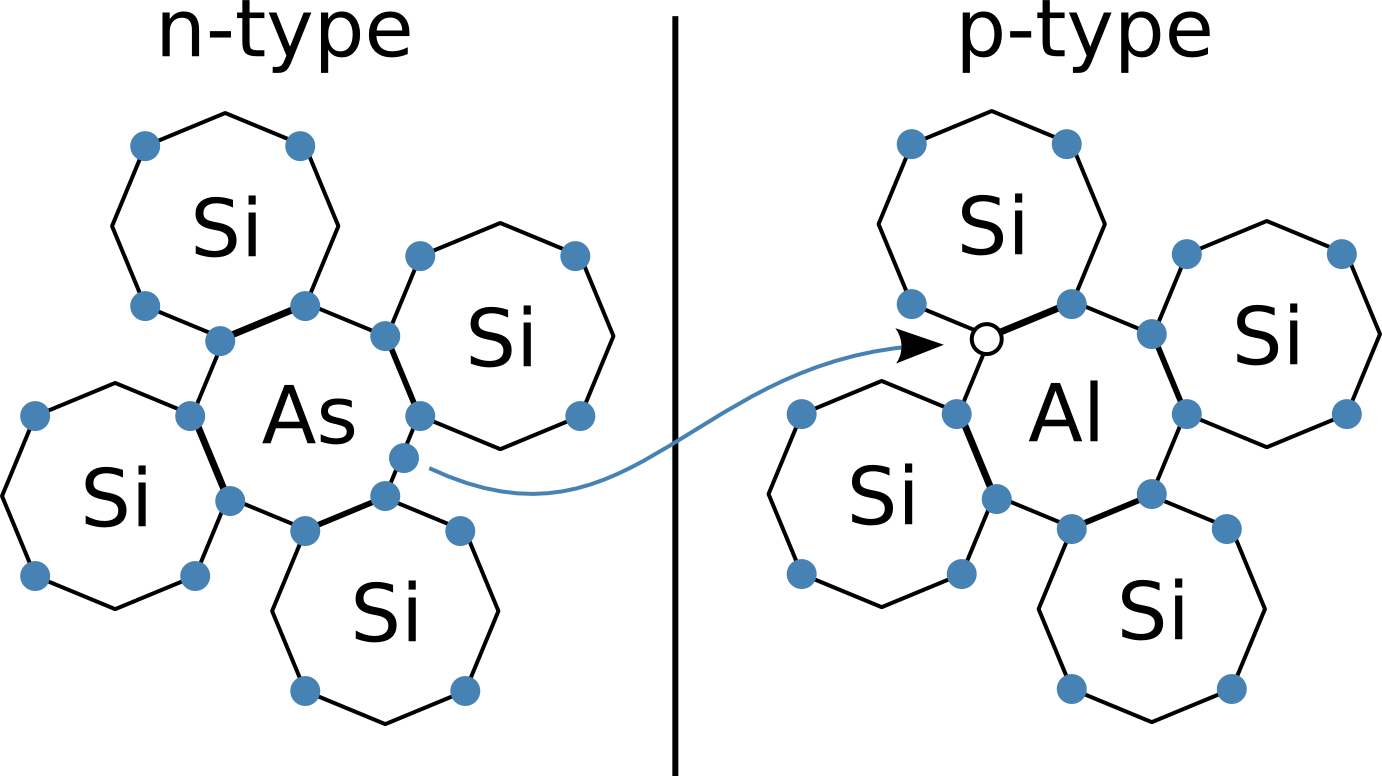
\includegraphics[width=\textwidth]{./img/krystall-pn}

\subsubsection{Sperresjikt}
Hvis man setter sammen n-type og p-type materialer,
vil det ved diffusjon trekkes elektroner
fra n-type over til p-type.
\\\\
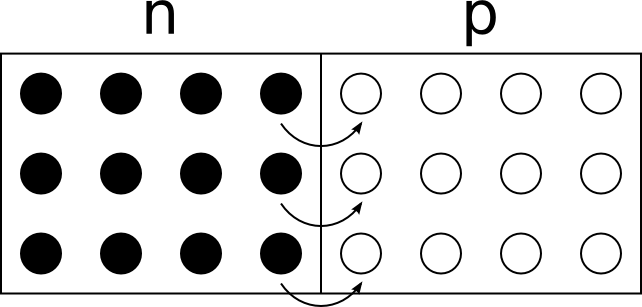
\includegraphics[width=0.67\textwidth]{./img/pn-junction}
\\\\
Elektronene \emph{rekombinerer} med hull på den andre siden,
og etterlater seg hull der de kom fra.
\\\\
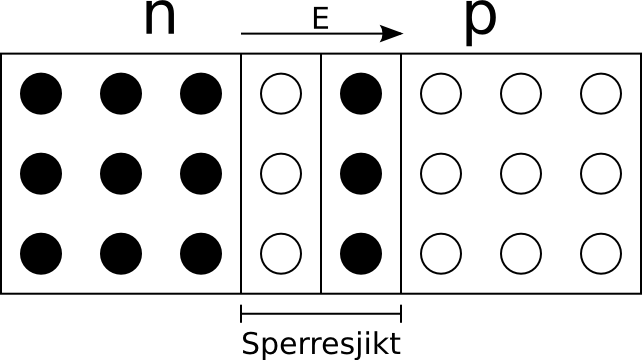
\includegraphics[width=0.67\textwidth]{./img/pn-sperresjikt}
\\
Det skapes et sperresjikt (depletion layer) mellom materialene.
Dette sjiktet fungerer som en isolator og stopper videre overføring.

\subsubsection{Forward bias}
TODO

\subsubsection{Reverse bias}
TODO
